\documentclass[12pt]{article}
\usepackage[a4paper, margin=.30in]{geometry}
\usepackage{graphicx ,
            wrapfig,
            xcolor, 
            enumerate,
            amsmath,fontenc
            }

\newcommand\headerMe[2]{\noindent{}#1\hfill#2}
\renewcommand{\thesection}{\Roman{section}}

\title{Leçon N 5 :Equilibre d’un corps solide soumis à deux forces }
\author{Zakaria HAOUZAN}
\date{\today}

\begin{document}
% headers --------------
\headerMe{Matière : Physique-Chimie}{Professeur : Zakaria HAOUZAN}\\
\headerMe{Unité : La Mécanique}{Établissement : Lycée SKHOR qualifiant}\\
\headerMe{Niveau : TCS}{Heure : 3H}\\

% ------Content ________
\begin{center}
    \Large{Leçon $N^{\circ}5$: \color{red} Equilibre d’un corps solide soumis à deux forces }
\end{center}

\begin{wrapfigure}{r}{0.2\textwidth}
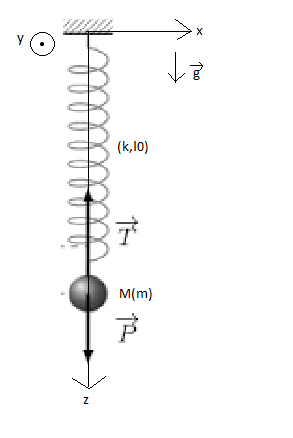
\includegraphics[width=0.2\textwidth]{./img/img00.png}
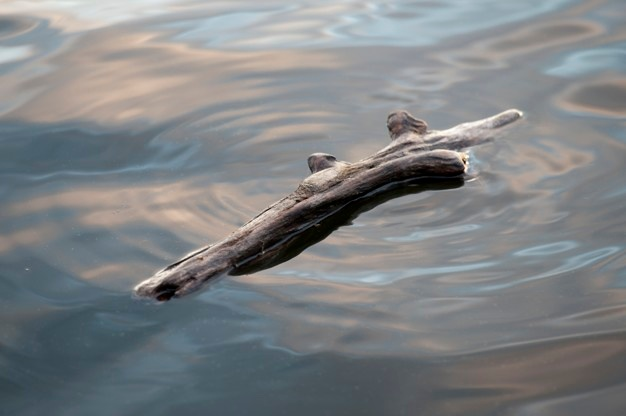
\includegraphics[width=0.2\textwidth]{./img/img01.jpg}
\end{wrapfigure}



\section{Questions : }

 - Donner un exemple d’un corps solide en équilibre, et soumis à 2 forces
 \\- Quels sont les conditions d’équilibre d’un corps solide soumis à 2 forces ?
\\- Quel est l’appareil qui permet de mesurer l’intensité d’une force ?
\\- Donner l’expression de la masse volumique et son unité dans le
(S.I)

\section{Situation problème : }

Le schéma (1) représente une masse marquée attaché à l’extrémité
d’un ressort. La masse marquée est en équilibre à cause d’une force
appliquée par le ressort
\\Le schéma (2) représente un morceau de bois flotte sur la surface de
l’eau. Le morceau de bois est en équilibre à cause d’une force
appliquée par l’eau
\\ - Que s’appelle la force appliquée par le ressort ? et quelles sont ses
caractéristiques ?
\\ - Que s’appelle la force appliquée par l’eau ? et quelles sont ses
caractéristiques ?


\section{ Rappel : Condition d’équilibre d'un corps solide sous l'action de deux forces}

Lorsqu’un corps est en équilibre sous l’action de deux forces $\vec{F_1}$ et $\vec{F_2}$, alors ces deux forces ont :

 - La même direction
 
 - Des sens opposés : $\vec{F_1} = \vec{F_2}$
 
 - La même intensité : $F_1 = F_2$

\section{Force exercée par un ressort : }
\subsection{Activité 1 }

%\begin{wrapfigure}{r}{0.3\textwidth}
%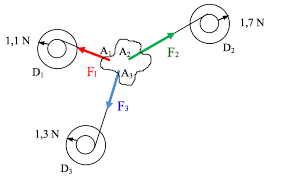
\includegraphics[width=0.3\textwidth]{./img/img01.png}
%\end{wrapfigure}

On attache à l’extrémité du ressort (de spires non jointives et de masse négligeable)
avec un support, la longueur initiale (à vide) du ressort est $l_0$, on suspend à l’autre
extrémité une masse marquée (S) de masse $m$, et on mesure chaque fois la longueur
finale l du ressort, Nous obtenons les résultats suivants :

\begin{center}
\begin{tabular}{ |c|c|c|c|c|c|c|c|c| }
 \hline
    m(g)         & 0  &  & & & & & & \\\hline
    l(cm)        &    &  & & & & & &  \\\hline
    T(N)         &    &  & & & & & &   \\\hline
    $\Delta(cm)$ &    &  & & & & & &    \\\hline
 \hline
\end{tabular}
\end{center}
\begin{enumerate}
        \item Faire l’inventaire des forces appliquées à la masse marquée (S), et les représenter sur la figure
        \item On applique la condition de l’équilibre, déterminer l’intensité de la force exercée par le ressort pour
chaque masse marquée
        \item On appelle allongement du ressort $\Delta{l}$ la différence entre la longueur finale l et la longueur initiale l0 :
            $\Delta{l} = |l - l_0|$  Compléter le remplissage du tableau
        \item Tracer la courbe de en fonction de $\Delta{l}$
        \item Trouver la relation entre l’intensité du ressort et l’allongement du ressort $\Delta{l}$
\end{enumerate}


\subsection{Conclusion : }
Lorsqu’on suspend un solide à un ressort, le ressort exerce une force sur le solide, appelée la tension du ressort $\vec{T}$ ,
ses caractéristiques sont :

  - Point d’application : point d’accroche du ressort

  - Direction : celle du ressort

  - Sens : opposée à la déformation du ressort

  - intensité : $T = k.\Delta{l} = k|l - l_0|$
  Avec la constante de raideur du ressort en $N.m^{-1}$
et l’allongement $\Delta{l}$ en m

\section{La poussée d'Archimède :  }

 
\subsection{Activité 2}

\begin{wrapfigure}{r}{0.3\textwidth}
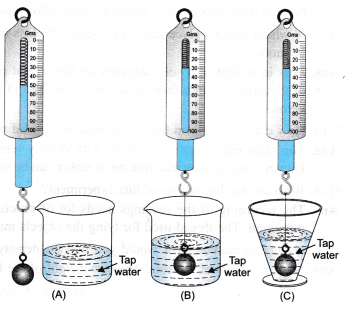
\includegraphics[width=0.3\textwidth]{./img/img03.png}
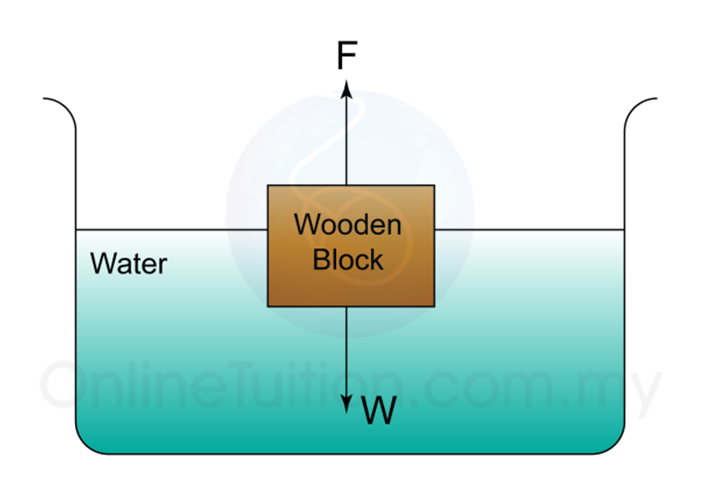
\includegraphics[width=0.3\textwidth]{./img/img04.png}
\end{wrapfigure}

On suspend le corps (S) à un ressort, et on verse l’eau dans une
éprouvette graduée

On immerge complètement le corps (S) dans l’eau

On donne : la masse volumique de l’eau : $\rho = 1g/{cm^3}$
Intensité de pesanteur g = 9.81 N/kg

\begin{enumerate}
    \item Faire l’inventaire des forces appliquées au corps (S) avant de l’immerger dans l’eau. Que représente la
valeur indiquée par le dynamomètre ?
    \item Faire l’inventaire des forces appliquées au corps (S) après de l’immerger dans l’eau
    \item Mesurer le volume de l’eau déplacée
    \item Calculer le poids de l’eau déplacée, et le Comparer avec l’intensité de poussée d’Archimède. Conclure

\end{enumerate}

\subsection{Conclusion :  }

La poussée d'Archimède $\vec{F_a}$ est une force de contact répartie exercée par un fluide (liquide ou gaz) sur un solide immergé, ses caractéristiques sont :

 - Point d’application : centre d’inertie de partie immergé
 
 - Direction : la verticale

 - Sens : vers le haut

 - Intensité : égale au poids de fluide déplacé $F_a = \rho g V$
 avec $\rho$ en $Kg.m^{-3}$ , V en $m^3$ et g en $N/Kg$

\end{document}
